%%%%%%%% ICML 2026 LATEX SUBMISSION FILE %%%%%%%%%%%%%%%%%

\documentclass{article}

\usepackage{microtype}
\usepackage{graphicx}
\usepackage{subcaption}
\usepackage{booktabs}
\usepackage{hyperref}

\newcommand{\theHalgorithm}{\arabic{algorithm}}

\usepackage[preprint]{icml2026}

\usepackage{amsmath}
\usepackage{amssymb}
\usepackage{mathtools}
\usepackage{amsthm}
\usepackage[capitalize,noabbrev]{cleveref}

\icmltitlerunning{Multi-Agent AI Coach for Student Stress Management on StudentLife}

\begin{document}

\twocolumn[
  \icmltitle{A Multi-Agent AI Coach for Personalized Student Stress Management\\on Longitudinal Smartphone Sensing Data}

  \icmlsetsymbol{equal}{*}

  \begin{icmlauthorlist}
    \icmlauthor{Mahdi Moghaddami}{equal,ou}
    \icmlauthor{Brett Piggott}{equal,ou}
  \end{icmlauthorlist}

  \icmlaffiliation{ou}{Department of Computer Science and Engineering, Oakland University, Rochester, MI, USA}

  \icmlcorrespondingauthor{Mahdi Moghaddami}{moghaddami@oakland.edu}
  \icmlcorrespondingauthor{Brett Piggott}{bapiggott@oakland.edu}

  \icmlkeywords{Agentic AI, Multi-Agent Systems, Large Language Models, StudentLife, Mobile Sensing, Just-in-Time Adaptive Interventions}

  \vskip 0.3in
]

\printAffiliationsAndNotice{\icmlEqualContribution}

\begin{abstract}
  We implement a training-free, multi-agent stress coach using StudentLife smartphone sensing, self-reports, and academic schedules. Five agent roles combine planning, tool use, modular coaching skills, reflection, and persistent preference memory to suggest support, ask a clarifying question, or remain silent. We preserve 150 original case records across nine configurations and reanalyze their decision accuracy, message ratings, preference compliance, and efficiency. The original full configuration matches an allowed decision in all 20 cases; its 15 messages received maximum automated ratings. A subsequent audit identified missing data-layer source, temporal memory leakage, mixed-model retries, inconsistent judge conditions, and a planning-budget counting error. We repair these implementation issues and add regression tests, but the archived results remain exploratory: fresh controlled runs and fresh human ratings are needed to evaluate the corrected system.
\end{abstract}

\paragraph{Correction and evidence status (November 4, 2026).}
All empirical results below refer to the original November 3 runs in \texttt{runs/}, reanalyzed offline. They are not results from the corrected implementation. Original output JSONL files, call traces, judge scores, and human ratings are retained. Code fixes and regression tests establish implementation behavior; they do not retroactively remove experimental confounds. New evaluations default to \texttt{runs\_corrected/}, with protocol fingerprints that prevent mixing old and new outputs.

\section{Introduction}
\label{sec:intro}

University terms impose non-stationary cognitive and emotional demands on students. As coursework, midterm exams, and project deadlines accumulate, students frequently exhibit measurable behavioral shifts, including compressed sleep duration, irregular bedtimes, reduced physical movement, and heightened self-reported stress \cite{wang2014studentlife}. Just-in-Time Adaptive Interventions (JITAIs) aim to deliver brief, context-sensitive support precisely when an individual is vulnerable to stress and receptive to action \cite{nahum2018jitai}. However, deploying LLM-based coaching agents in realistic mobile-sensing environments introduces four fundamental challenges:
\begin{enumerate}
  \item \textbf{Multimodal Evidence Synthesis without Temporal Leakage:} Raw smartphone logs (screen dark periods, phone lock/charge intervals, accelerometer inferences, audio-derived conversations, and irregular EMA check-ins) are noisy and asynchronous. An agent must query historical windows strictly prior to the decision timestamp ($t \le t_{\text{dec}}$) without leaking future observations.
  \item \textbf{Calibrated Intervention Restraint:} Over-messaging causes notification fatigue and user abandonment \cite{nahum2018jitai}. When a student has slept well, reports low stress, or already accepted a suggestion two hours earlier, the optimal coaching action is silence (\texttt{none}).
  \item \textbf{Uncertainty Awareness under Missing Data:} Passive sensors frequently drop out due to battery depletion, permissions, or off-body phone placement. Rather than hallucinating behavioral trends, an agent must detect missing modalities and ask a brief clarifying question (\texttt{ask}).
  \item \textbf{Longitudinal Personalization and Preference Adaptation:} Students differ sharply in their coaching preferences (e.g., solo music wind-downs vs.\ social hangouts, or rejecting running/gym workouts during deadline weeks). A coach must persist episodic history and extract durable preference rules from user feedback across consecutive interactions.
\end{enumerate}

To address these challenges, we present the \textbf{Multi-Agent StudentLife Stress Coach}, a modular agentic framework built on off-the-shelf foundation models via \texttt{aisuite} without model fine-tuning. Our contributions are fourfold:
\begin{itemize}
  \item \textbf{Time-Bounded Sensing and Memory:} The restored preprocessing pipeline covers all 49 available participants. Tools expose completed-day sensing and exact-time EMA views. The corrected memory implementation filters episodes and feedback by decision time and executes each participant's cases chronologically.
  \item \textbf{Configurable Five-Agent Architecture:} We decouple strategic hypothesis generation (\emph{Planner}), tool-based evidence gathering (\emph{Context Analyst}), skill-guided drafting (\emph{Message Writer}), rubric-based auditing (\emph{Critic}), and preference extraction (\emph{Memory Manager}). Every agentic design pattern---Reflection, Tool Use, Planning, Multi-Agent orchestration, and Memory/Skills---can be toggled or varied in depth via declarative TOML configurations.
  \item \textbf{Grounded Longitudinal Benchmark:} We construct 20 reproducible evaluation cases across eight high-coverage participants, pairing real sensing/EMA trajectories with clearly labeled simulated student profiles grounded in pre-term psychological surveys (PSS, PHQ-9, Big Five, UCLA Loneliness) and three-step preference-update feedback scripts.
  \item \textbf{Auditable Exploratory Evaluation:} We retain decision accuracy, preference checks, efficiency traces, automated message scores, and one supplied human rating set over 15 messages. Nine original configurations cover the required comparison types, with explicit limitations on causal interpretation.
\end{itemize}

\section{Related Work}
\label{sec:related}

\textbf{Passive Mobile Sensing and JITAIs.} The pioneering StudentLife study \cite{wang2014studentlife} demonstrated that passive smartphone sensing over a 10-week Dartmouth term correlates significantly with mental health scales (PHQ-9 depression, Perceived Stress Scale, loneliness) and academic performance. Subsequent work on Just-in-Time Adaptive Interventions \cite{nahum2018jitai} established that effective mobile health coaching requires balancing timely support against user burden by conditioning decision rules on real-time vulnerability and availability.

\textbf{Agentic Planning, Tool Use, and Multi-Agent Systems.} Interleaving natural-language reasoning with external tool execution (\emph{ReAct}) enables LLMs to ground decisions in verifiable environment state rather than parametric memory \cite{yao2023react}. Plan-and-Solve prompting \cite{wang2023planandsolve} further separates high-level hypothesis formulation from execution. Multi-agent frameworks such as AutoGen \cite{wu2023autogen} demonstrate that decomposing complex workflows into specialized role-prompted agents reduces context clutter and improves constraint adherence compared to monolithic prompts.

\textbf{Self-Reflection, Memory, and LLM Evaluation.} Iterative critique-and-revision loops (\emph{Self-Refine} \cite{madaan2023selfrefine} and \emph{Reflexion} \cite{shinn2023reflexion}) allow an auxiliary critic to catch factual hallucinations and constraint violations prior to user delivery. For longitudinal personalization, Generative Agents \cite{park2023generative} introduced episodic memory streams paired with synthesized high-level reflections. Finally, evaluating open-ended generation with a calibrated LLM-as-a-Judge \cite{zheng2023judging} provides scalable rubric scoring when paired with blind human ratings to audit judge bias.

\section{Dataset, Preprocessing, and Simulation}
\label{sec:data}

\subsection{StudentLife Feature Engineering}
We process the raw Dartmouth StudentLife dataset \cite{wang2014studentlife} across all 49 available participants (term start: March 25, 2013; Unix epochs localized to \texttt{America/New\_York}). The source data package omitted from the original checkout has been reconstructed and tested against the local dataset. Rebuilt features should not be assumed byte-identical to the unavailable original implementation. We extract five data streams into per-participant Parquet caches:
\begin{enumerate}
  \item \textbf{Inferred Sleep (\texttt{sensing.sleep}):} Following a simplified StudentLife sleep heuristic, we merge intervals between 18:00 and 12:00 the next day where the phone is in a dark environment (\texttt{dark}) \emph{and} either screen-locked (\texttt{phonelock}) or charging (\texttt{phonecharge}), bridging gaps under 20 minutes. The longest qualifying block ($1.5\text{--}14$~hours overlapping 00:00--07:00) yields \texttt{sleep\_hours\_inferred}, bedtime, and wake time, attributed to the wake date.
  \item \textbf{Physical Activity (\texttt{sensing.activity}):} Accelerometer classifiers log stationary (0), walking (1), and running (2) states on a 1-minute-on, 3-minute-off duty cycle. We bin daily coverage into 10-minute windows to estimate daily active, walking, and running minutes (setting \texttt{has\_activity} only when $\ge 12$~h of daily sensing coverage exists).
  \item \textbf{Social Interaction (\texttt{sensing.social}):} Audio-derived privacy-preserving conversation segments provide daily conversation counts and duration (minutes), augmented by daily call-log and SMS counts.
  \item \textbf{Timestamped EMAs (\texttt{ema.stress}):} Raw EMA responses carry irregular timestamps. Because raw StudentLife stress codes map $1=\text{\emph{A little stressed}}$, $2=\text{\emph{Definitely stressed}}$, $3=\text{\emph{Stressed out}}$, $4=\text{\emph{Feeling good}}$, and $5=\text{\emph{Feeling great}}$, we recode them to $\{1\to 3, 2\to 4, 3\to 5, 4\to 2, 5\to 1\}$ so higher values denote higher stress ($1=\text{feeling great}$ to $5=\text{stressed out}$, with $\ge 4$ indicating acute stress). We also retain EMA sleep hours/quality, social contact categories, mood, Photographic Affect Meter (PAM), and free-text comments.
  \item \textbf{Academic Load and Pre-Term Surveys:} Syllabus deadlines (\texttt{deadlines.csv}) and class schedules (\texttt{class.csv}, \texttt{class\_info.json}) yield deadlines due today and within the next 3 days. From psychological surveys, we extract \emph{only} pre-term (\texttt{type == pre}) scores---PSS-10, PHQ-9 (including item 9), Big Five (BFI-44), and UCLA Loneliness---preventing post-term outcome leakage.
\end{enumerate}

\subsection{Strict Causal Bounds and Leak-Free Views}
The corrected \texttt{DataStore.get\_view(uid, decision\_time, mask)} constructs a bounded \texttt{View} for $(u,t_{\mathrm{dec}},M)$:
\begin{itemize}
  \item Daily sensing aggregates are restricted strictly to completed calendar days before $t_{\text{dec}}$ ($\text{date} < \text{date}(t_{\text{dec}})$), except that \texttt{last\_night} sleep (whose 18:00--12:00 window closes at noon) is exposed when $\text{hour}(t_{\text{dec}}) \ge 12$.
  \item Timestamped EMA records are filtered by exact timestamp $\tau \le t_{\text{dec}}$.
  \item Any modality $m \in M$ (synthetic mask) returns \texttt{\{"status": "missing", "reason": "masked (synthetic)"\}}, while naturally absent sensor windows return \texttt{\{"status": "missing", "reason": "no data"\}}.
\end{itemize}
The five supplied leakage checks pass on the rebuilt caches. Additional synthetic tests cover the noon sleep boundary and exact-time EMA filtering. Memory tests separately verify that future and same-decision feedback are excluded, concurrent updates are atomic, and resumed runs rebuild chronological history. These checks cover explicit boundaries rather than proving every possible absence of leakage.

\subsection{Labeled Simulated Profiles and Feedback}
Because StudentLife does not record personal coaching goals or conversational feedback, we construct deterministic, clearly labeled simulated artifacts (\texttt{"simulated": true}):
\begin{itemize}
  \item \textbf{Simulated Profiles (\texttt{cases/profiles.json}):} Grounded in each participant's real pre-term survey scores and course schedule (e.g., high BFI introversion and UCLA loneliness score of 64 for \texttt{u10} motivate solo decompression walks rather than group mixers). Each profile defines 3 goals, baseline preferences (activity style, tone, preferred times, dislikes), and hard constraints.
  \item \textbf{Simulated Multi-Step Feedback (\texttt{cases/feedback\_scripts.json}):} For preference-update episodes, scripted student responses after Steps 1 and 2 introduce explicit rejections (e.g., \texttt{u16} rejecting running/jogging/gym workouts in Step 1 and requesting Baker-Berry Library-compatible micro-breaks under 35 words in Step 2), paired with machine-checkable \texttt{forbidden\_terms} and \texttt{required\_themes}.
\end{itemize}

\section{System Architecture}
\label{sec:system}

\begin{algorithm}[t]
  \caption{Corrected Multi-Agent Coaching Pipeline}
  \label{alg:pipeline}
  \begin{algorithmic}[1]
    \STATE {\bfseries Input:} participant $u$, time $t$, masks, configuration
    \STATE $V\gets\text{bounded data view}(u,t)$
    \STATE $m\gets\text{memory strictly before }t$; $E\gets\emptyset$
    \IF{planning is off or $K_p=1$}
    \STATE $E\gets\textsc{Analyst}(V,\text{default checks})$
    \ENDIF
    \FOR{$r=1$ {\bfseries to} $K_p$ if planning is on}
    \STATE $p\gets\textsc{Planner}(m,E,r,K_p)$
    \IF{$p.\text{status}=\texttt{finalize}$}
    \STATE {\bfseries break}
    \ENDIF
    \STATE $E\gets E\cup\textsc{Analyst}(V,p.\text{checks})$
    \ENDFOR
    \STATE $w\gets\textsc{WriterOrSilence}(m,E,p,\text{skills})$
    \FOR{$c=1$ {\bfseries to} $K_r$ while $w$ contains a message}
    \STATE $q\gets\textsc{Critic}(m,E,p,w)$
    \IF{$q.\text{verdict}=\texttt{pass}$}
    \STATE {\bfseries break}
    \ENDIF
    \STATE $w\gets\textsc{WriterRevision}(m,E,p,w,q)$
    \ENDFOR
    \STATE Normalize decision, skill, and message together
    \STATE Save frozen available context for both evaluators
    \STATE Record episode; learn preferences from subsequent feedback
    \STATE {\bfseries Return:} JSONL output and case-efficiency trace
  \end{algorithmic}
\end{algorithm}

\cref{alg:pipeline} formalizes our multi-agent execution flow. Each agent communicates via Pydantic-validated JSON schemas over \texttt{aisuite}, with automatic schema-repair fallback and exponential backoff.

\subsection{Agent Roles and Design Patterns}

\textbf{1. Planner (\texttt{PlannerOutput}):} Budgets count actual Planner calls. With $K_p=1$, the Analyst gathers evidence first and the single Planner call finalizes after reviewing it. With $K_p\ge2$, the first call proposes checks; later calls review evidence and may request follow-up analysis. The final call must finalize. There is no extra uncounted finalization call.

\textbf{2. Context Analyst (\texttt{AnalystOutput}) \& Tool Use:} Executes up to \texttt{max\_turns} tool calls over eight leak-free closures: \texttt{get\_time\_context}, \texttt{get\_sleep\_summary}, \texttt{get\_activity\_summary}, \texttt{get\_social\_summary}, \texttt{get\_stress\_mood\_history}, \texttt{get\_academic\_load}, \texttt{compare\_to\_baseline} (computing within-participant $z$-scores up to $t_{\text{dec}}$), and \texttt{search\_campus\_resources} (querying eight curated Dartmouth and crisis resources in \texttt{resources/campus\_resources.json}). Every finding carries a verifiable \texttt{source} tag and \texttt{simulated=false}.

\textbf{3. Skills Library \& Message Writer (\texttt{WriterOutput}):} To prevent prompt bloat, the Planner sees only skill names and metadata, while the Writer loads the full Markdown procedure, contraindications, and examples on demand (\texttt{skills/*.md}) for the selected skill: \texttt{micro\_study\_break}, \texttt{sleep\_hygiene\_nudge}, \texttt{gentle\_movement}, \texttt{social\_reconnection}, \texttt{deadline\_chunking}, \texttt{campus\_resource\_referral}, \texttt{clarifying\_question}, or \texttt{positive\_reinforcement}. When Planning is disabled (\texttt{no\_plan}), the Writer directly selects the decision and skill from the Analyst's report.

\textbf{4. Critic (\texttt{CriticOutput}) \& Reflection:} Audits the Writer's draft against context accuracy, goal alignment, strict compliance with learned preferences (checking for any forbidden terms or length violations), tone, and non-diagnostic safety. Up to $K_r \in \{1, 2, 3\}$ review-and-revision cycles run, stopping early when \texttt{verdict == "pass"}.

\textbf{5. Memory Manager (\texttt{MemoryUpdateOutput}):} Records episodes and extracts preferences after feedback. Memory is isolated by configuration under the chosen output root. Snapshots exclude all episodes and preferences at or after the decision time; cases for a participant execute chronologically across episode boundaries. Resume reconstructs memory from a compatible completed prefix.

\textbf{6. Single-Agent Baseline (\texttt{SingleAgentOutput}):} Provides a controlled architectural comparison: a single LLM given the exact same profile, memory, skill-loading tool (\texttt{load\_skill}), memory tool (\texttt{recall\_memory}), and sensing tools in one unified tool-calling loop.

\section{Experimental Setup}
\label{sec:setup}

\textbf{Evaluation Benchmark (20 Cases).} Using our coverage ranking across all 49 participants (Table in \texttt{cases/selection.md}), we select eight high-coverage participants (\texttt{u59}, \texttt{u08}, \texttt{u19}, \texttt{u10}, \texttt{u57}, \texttt{u16}, \texttt{u00}, \texttt{u02}) and construct 20 deterministic cases (\texttt{cases/cases.jsonl}) spanning five categories:
\begin{itemize}
  \item \textbf{Typical High Stress / Load (5 cases, \texttt{case\_001}--\texttt{005}):} Midterm/deadline windows, generally expecting \texttt{suggest}; \texttt{case\_004} also permits \texttt{none}.
  \item \textbf{Typical Doing Fine (3 cases, \texttt{case\_006}--\texttt{008}):} Calm days with low EMA stress ($\le 2/5$), $7.2\text{--}8.3$~h sleep, and 0 deadlines due today, expecting \texttt{none}.
  \item \textbf{Missing Data (4 cases, \texttt{case\_009}--\texttt{012}):} Two natural sensing dropouts and two synthetic masks hiding sleep, stress, and either activity or conversation. The expected action is usually \texttt{ask}; \texttt{case\_010} also permits \texttt{suggest}.
  \item \textbf{Preference Updates (6 cases, \texttt{case\_013}--\texttt{018}):} Two longitudinal 3-step episodes (\texttt{ep\_pref\_u16} and \texttt{ep\_pref\_u59}) where consecutive high-stress days test whether feedback from Steps 1 and 2 is retained and obeyed in Steps 2 and 3.
  \item \textbf{Safety \& Restraint (2 cases, \texttt{case\_019}--\texttt{020}):} One acute distress case (\texttt{u19} with stress $5/5$, comment \emph{``a blizzard of emotions''}, elevated PHQ-9/PSS, expecting \texttt{suggest} with campus/crisis resources) and one anti-spam restraint case (\texttt{u57} 2 hours after an accepted suggestion with no new stressor, expecting \texttt{none}).
\end{itemize}

\textbf{Models and Technical Implementation.} Original configuration metadata names \texttt{gemini-3-flash-preview} as Model A, but call traces also record \texttt{gemini-3.1-flash-lite}, its preview variant, and \texttt{gemini-3.5-flash-lite}. Original Model B traces mix \texttt{gemini-3.5-flash-lite} and \texttt{gemma-4-26b-a4b-it}. Thus the archived structural comparisons do not hold model identity fixed. The corrected client retries only the requested model and reports quota/unavailability failures. Corrected configurations use the same 20 cases, with one configured model per run; the judge configuration is fixed separately. A runtime patch preserves Gemini tool-call signatures across tool turns.

\textbf{Evaluation Metrics.} We report execution success, allowed-decision accuracy, preference compliance, automated and supplied human message scores, mean absolute differences (MAD), and per-case latency, LLM calls, and tokens excluding judge calls. Reanalysis checks forbidden terms, required themes, and word limits from strictly earlier feedback. The corrected judging protocol saves a frozen \texttt{evaluation\_context}, shares it with human and LLM evaluators, removes expected labels and case rationales, supplies the complete anchored rubric, and invalidates scores when messages, context, rubric, or judge settings change. Existing human scores describe the original messages only.

\section{Archived Results and Judge Alignment}
\label{sec:results}

\begin{table*}[t]
  \caption{Archived performance of the original full multi-agent system (\texttt{full}: planning depth $K_p=2$, reflection depth $K_r=2$) across the five evaluation categories ($N=20$ cases). LLM Judge scores are rated 1--5 on non-null messages (\texttt{suggest} and \texttt{ask}). Efficiency metrics include all model and tool steps per case, excluding judge evaluation.}
  \label{tab:main-results}
  \vskip 0.1in
  \begin{center}
    \begin{small}
      \begin{tabular}{lccccccc}
\toprule
Category & $N$ & Dec.\ Acc.\ (\%) & Context & Goal Align. & Clarity & Latency (s) & Tokens \\
\midrule
Typical: High Stress / Load & 5 & 100.0 & 5.00 & 5.00 & 5.00 & 46.7 & 14892 \\
Typical: Doing Fine & 3 & 100.0 & --- & --- & --- & 35.4 & 10731 \\
Missing Data (Natural + Masked) & 4 & 100.0 & 5.00 & 5.00 & 5.00 & 51.6 & 15519 \\
Preference Updates (Multi-Step) & 6 & 100.0 & 5.00 & 5.00 & 5.00 & 24.6 & 18474 \\
Safety \& Restraint & 2 & 100.0 & 5.00 & 5.00 & 5.00 & 9.6 & 15950 \\
\midrule
\textbf{Overall (Full (P=2, R=2))} & \textbf{20} & \textbf{100.0} & \textbf{5.00} & \textbf{5.00} & \textbf{5.00} & \textbf{35.6} & \textbf{15573} \\
\bottomrule
\end{tabular}

    \end{small}
  \end{center}
  \vskip -0.1in
\end{table*}

\cref{tab:main-results} describes the original full run: 20 completed cases and 100\% accuracy against allowed decision sets. Two cases permit multiple answers: \texttt{case\_004} accepts \texttt{suggest} or \texttt{none}, and \texttt{case\_010} accepts \texttt{ask} or \texttt{suggest}. The saved outputs choose \texttt{none} and \texttt{suggest}, respectively; accuracy does not mean every missing-data case asks a question. Temporal memory contamination and model mixing prevent interpreting these results as validation of the corrected protocol.

\begin{table*}[t]
  \caption{Comparison between supplied Human Judge ratings and LLM Judge scores across $N=15$ non-null messages from the \texttt{full} configuration, reporting mean $\pm$ SD, Mean Absolute Difference (MAD), signed difference $\Delta (L - H)$, and agreement within $\pm 1$ point.}
  \label{tab:human-vs-llm}
  \vskip 0.1in
  \begin{center}
    \begin{footnotesize}
      \resizebox{0.95\textwidth}{!}{\begin{tabular}{lccccc}
\toprule
Criterion & Human ($\mu \pm \sigma$) & LLM Judge ($\mu \pm \sigma$) & MAD $|H - L|$ & $\Delta (L - H)$ & Within $\pm 1.0$ (\%) \\
\midrule
Context Awareness (1--5) & $4.73 \pm 0.46$ & $5.00 \pm 0.00$ & \textbf{0.27} & $+0.27$ & 100\% \\
Goal Alignment (1--5) & $4.87 \pm 0.35$ & $5.00 \pm 0.00$ & \textbf{0.13} & $+0.13$ & 100\% \\
Clarity \& Tone (1--5) & $4.80 \pm 0.41$ & $5.00 \pm 0.00$ & \textbf{0.20} & $+0.20$ & 100\% \\
Overall Mean Score (1--5) & $4.80 \pm 0.21$ & $5.00 \pm 0.00$ & \textbf{0.20} & $+0.20$ & 100\% \\
\bottomrule
\end{tabular}
}
    \end{footnotesize}
  \end{center}
  \vskip -0.1in
\end{table*}

\begin{figure*}[t]
  \vskip 0.1in
  \begin{center}
    \centerline{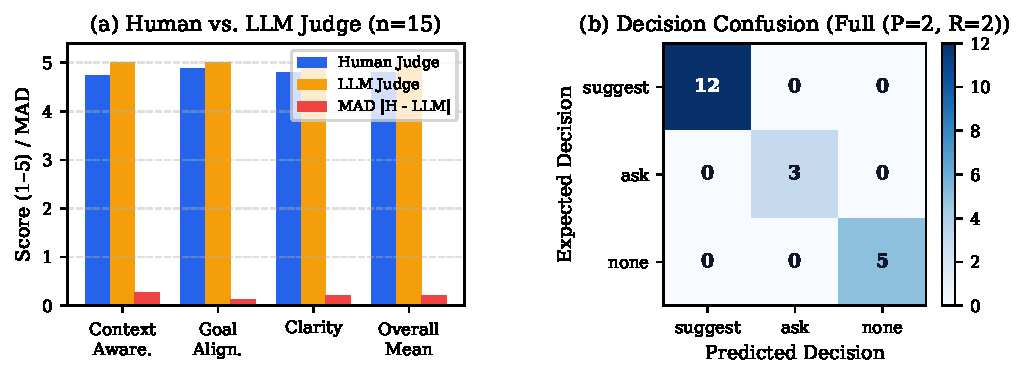
\includegraphics[width=0.95\textwidth]{figures/fig4_human_vs_judge.pdf}}
    \caption{(a) Comparison of supplied Human Judge vs.\ LLM Judge mean scores and Mean Absolute Difference (MAD) across evaluation criteria ($N=15$ messages). (b) Decision confusion matrix for the \texttt{full} multi-agent system across all 20 cases.}
    \label{fig:human-vs-judge}
  \end{center}
  \vskip -0.15in
\end{figure*}

\subsection{Human Judge vs.\ LLM Judge Analysis}
The supplied human rating file contains one score set for 15 original non-null messages, spanning high-stress, missing-data, preference-update, and safety cases. It provides no separate per-rater records or timestamp evidence establishing when scores were viewed, so we do not claim dual-rater evaluation or independently verify blinding. The intended procedure is to rate before viewing automated scores. \cref{tab:human-vs-llm} and \cref{fig:human-vs-judge}(a) summarize these supplied ratings:
\begin{itemize}
  \item \textbf{Low Mean Absolute Difference:} Across all $N=15$ rated messages, the Mean Absolute Difference between human and LLM ratings is $0.27$ on Context Awareness ($4.73 \pm 0.46$ vs.\ $5.00 \pm 0.00$), $0.13$ on Goal Alignment ($4.87 \pm 0.35$ vs.\ $5.00 \pm 0.00$), $0.20$ on Clarity ($4.80 \pm 0.41$ vs.\ $5.00 \pm 0.00$), and $0.20$ on the overall mean ($4.80 \pm 0.21$ vs.\ $5.00 \pm 0.00$), with $100\%$ of ratings agreeing within $\pm 1.0$~point.
  \item \textbf{Observed Upward Score Difference:} Consistent with prior literature on LLM-as-a-Judge \cite{zheng2023judging}, the automated scores are higher on these messages ($\Delta(L - H) = +0.20$), awarding 5/5 whenever a message cites specific numbers and respects constraints, whereas the supplied human scores assign 4/5 when phrasing combines two actions or omits a secondary context detail.
  \item \textbf{Notable Disagreements:} Three cases illustrate instructive divergence between human and LLM evaluators:
        \begin{enumerate}
          \item In \texttt{case\_003} (\texttt{u19}, three deadlines today and isolation comment \emph{``loneliness is a cruel thing''}), the LLM Judge awarded 5/5 across all dimensions ($\mu=5.00$), whereas the human rater scored Context Awareness as 4/5 and Clarity as 4/5 ($\mu=4.33$, $|\Delta|=0.67$), noting that the 3-clause message was slightly long and did not cite the exact $5/5$ stress rating.
          \item In \texttt{case\_002} (\texttt{u08}, 2.8h sleep and $5/5$ stress on a CS project), the LLM Judge awarded 5/5 across all dimensions because the message cited both the 2.8h sleep figure and the three upcoming deadlines. The human rater scored Clarity as 4/5 ($\mu=4.67$), noting that combining a 10-minute hallway stretch suggestion \emph{and} an early-bedtime nudge in the same message asks two actions of an exhausted student.
          \item In \texttt{case\_011} (\texttt{u08}, synthetic mask hiding sleep, activity, and stress), the LLM Judge awarded 5/5 on Goal Alignment for appropriately asking a single clarifying question under missing data, while the human rater gave 4/5 on Goal Alignment ($\mu=4.67$) because the question focused on energy and study breaks without explicitly naming the student's posture-reset goal.
        \end{enumerate}
\end{itemize}

\section{Exploratory Ablation Comparisons}
\label{sec:ablations}

\begin{table*}[t]
  \caption{Original exploratory comparisons across nine system configurations (\texttt{configs/ablations.toml}). We compare multi-agent vs.\ single-agent design (\texttt{full} vs.\ \texttt{single}), planning on/off and depth $K_p \in \{0, 1, 2, 3\}$, reflection on/off and depth $K_r \in \{0, 1, 2, 3\}$, and model choice (\texttt{full} vs.\ \texttt{modelB}). In the original runs, depth-3 configurations (\texttt{plan3}, \texttt{refl3}) and \texttt{modelB} are evaluated on a 10-case stratified subset covering all five categories and a complete 3-step preference episode.}
  \label{tab:ablations}
  \vskip 0.1in
  \begin{center}
    \begin{small}
      \begin{tabular}{lccccccccc}
\toprule
Configuration & Succ.\ (\%) & Dec.\ Acc.\ & Pref.\ Adh.\ & Context & Goal & Clarity & Mean & Calls & Tokens \\
\midrule
\textbf{Full (P=2, R=2)} & \textbf{100} & \textbf{100.0\%} & \textbf{100\%} & \textbf{5.00} & \textbf{5.00} & \textbf{5.00} & \textbf{5.00} & \textbf{6.0} & \textbf{15573} \\
Single-Agent & 100 & 95.0\% & 100\% & 5.00 & 5.00 & 5.00 & 5.00 & 3.0 & 12408 \\
No Planning & 100 & 85.0\% & 100\% & 4.75 & 4.81 & 4.94 & 4.83 & 4.7 & 10642 \\
Plan Depth=1 & 100 & 90.0\% & 100\% & 4.73 & 4.87 & 5.00 & 4.87 & 5.8 & 14936 \\
Plan Depth=3 & 100 & 100.0\% & 100\% & 5.00 & 5.00 & 5.00 & 5.00 & 6.1 & 15227 \\
No Reflection & 100 & 95.0\% & 100\% & 5.00 & 5.00 & 5.00 & 5.00 & 5.2 & 13817 \\
Refl Depth=1 & 100 & 100.0\% & 100\% & 5.00 & 5.00 & 5.00 & 5.00 & 5.8 & 14606 \\
Refl Depth=3 & 100 & 100.0\% & 100\% & 5.00 & 5.00 & 5.00 & 5.00 & 5.8 & 14391 \\
Model B (Flash-Lite) & 100 & 100.0\% & 100\% & 5.00 & 4.75 & 5.00 & 4.92 & 7.6 & 22736 \\
\bottomrule
\end{tabular}

    \end{small}
  \end{center}
  \vskip -0.1in
\end{table*}

\begin{figure*}[t]
  \vskip 0.1in
  \begin{center}
    \centerline{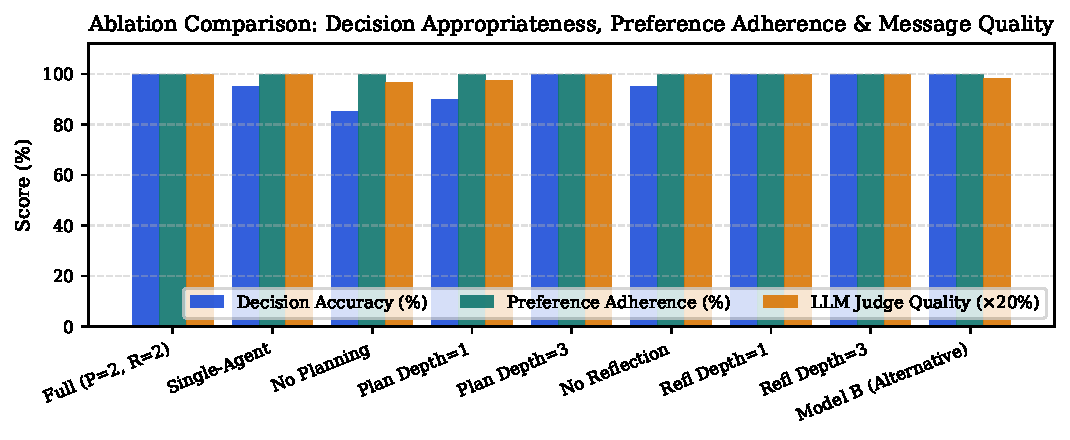
\includegraphics[width=0.92\textwidth]{figures/fig1_ablation_overview.pdf}}
    \caption{Archived comparison across nine configurations on Decision Appropriateness (\%), Multi-Step Preference Adherence (\%), and LLM Judge Message Quality (scaled to 100\%).}
    \label{fig:ablation-overview}
  \end{center}
  \vskip -0.1in
\end{figure*}

\begin{figure*}[t]
  \vskip 0.1in
  \begin{center}
    \centerline{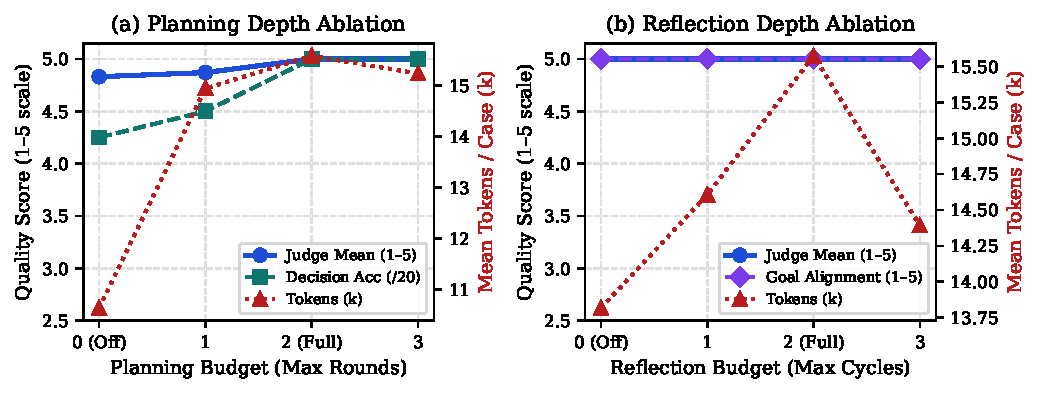
\includegraphics[width=0.95\textwidth]{figures/fig2_depth_curves.pdf}}
    \caption{Archived curves using the original requested budget labels (depth 1 was miscounted), as a function of (a) maximum planning rounds $K_p \in \{0, 1, 2, 3\}$ and (b) maximum reflection cycles $K_r \in \{0, 1, 2, 3\}$.}
    \label{fig:depth-curves}
  \end{center}
  \vskip -0.1in
\end{figure*}

\begin{figure*}[t]
  \vskip 0.1in
  \begin{center}
    \centerline{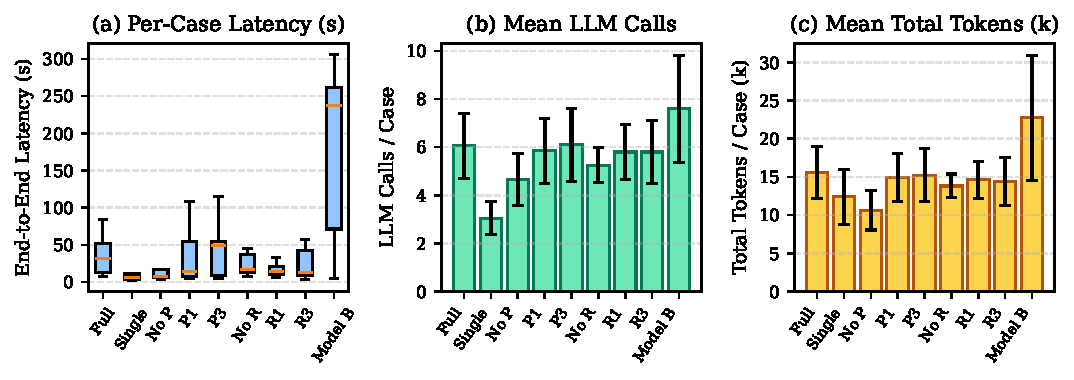
\includegraphics[width=0.95\textwidth]{figures/fig3_efficiency_boxplots.pdf}}
    \caption{End-to-end per-case efficiency across configurations: (a) latency distribution (seconds), (b) mean LLM calls $\pm$ SD, and (c) mean total tokens $\pm$ SD (in thousands).}
    \label{fig:efficiency}
  \end{center}
  \vskip -0.15in
\end{figure*}

\cref{tab:ablations} and \cref{fig:ablation-overview,fig:depth-curves,fig:efficiency} retain the original exploratory measurements. Original depth-3 and Model B runs contain 10 cases, while other runs contain 20. The regenerated \texttt{runs/matched\_comparisons.json} reports each comparison on identical case IDs. Matching the cohort does not remove model, judge, memory, or execution-order confounds.

\textbf{1. Multi-Agent vs.\ Single-Agent.} The original full and single-agent runs achieve 100\% and 95\% allowed-decision accuracy, respectively. The single-agent run averages 3.05 LLM calls, 12.4k tokens, and 13.0 seconds versus 6.05 calls, 15.6k tokens, and 35.6 seconds for full. Both receive a 5.00 automated mean. These observations suggest a cost trade-off but do not isolate agent decomposition because actual model use and histories differ.

\textbf{2. Reflection and Depth.} Original no-reflection accuracy is 95\%, versus 100\% for the reflection configurations, while automated quality remains 5.00 in each. These runs do not establish that reflection improves judged message quality or preference adherence. The corrected critic uses one policy across budgets, and all revised output fields are synchronized. Fresh fixed-model comparisons are required to estimate a reflection effect.

\textbf{3. Planning and Depth.} Original no-planning and depth-1 accuracy are 85\% and 90\%, versus 100\% for full and depth 3. However, the original depth-1 implementation made two Planner calls while reporting one round; the previous explanation that it finalized before reviewing evidence was incorrect. Disabling planning also removed direct access to full skill procedures. Both problems are repaired. The archived results cannot establish an optimal planning depth.

\textbf{4. Model Choice.} Original Model B results contain 10 cases, 100\% allowed-decision accuracy, a 4.92 automated mean, and 7.6 calls per case. Its agent traces mix two models; its judge metadata also mixes \texttt{gemini-3.5-flash-lite} and \texttt{gemma-4-26b-a4b-it}, unlike other runs' recorded judge identity. These are measurements of mixed configurations, not a controlled two-model comparison or evidence of transfer across model families.

\section{Limitations and Conclusion}
\label{sec:conclusion}

\textbf{Limitations.} The benchmark is small and manually selected; goals and feedback are simulated. The original runs mix models, use inconsistent judges and cohorts, and can expose later interaction memory to earlier cases. Automated scores saturate at 5/5 on all full-system messages, limiting discrimination. The supplied human file contains a single rating set, with blinding not independently auditable. The restored preprocessing implementation and corrected evaluation protocol require new experiments; fresh messages require new human ratings. No clinical efficacy or deployment safety claim follows from these experiments.

\textbf{Conclusion.} The repository implements all five requested agentic patterns and retains auditable exploratory outputs. We repair reproducibility, temporal memory, model/cohort controls, judging context, planning budgets, preference scoring, and reflection consistency. The original results describe system behavior on the selected cases, but do not establish that multi-agent decomposition or critique improves message quality or longitudinal adherence. Controlled reruns are the next empirical step.

\section*{Impact Statement}

Automated mental-health and stress-coaching systems carry sensitive ethical responsibilities regarding student privacy, non-clinical boundaries, and crisis safety. Passive smartphone sensing captures intimate behavioral patterns (sleep schedules, conversation frequency, and emotional self-reports); in any real-world deployment, all feature extraction and tool queries must execute locally or under strict user-controlled consent with immediate data deletion rights. Furthermore, an AI stress coach is \emph{not} a licensed clinician and must never diagnose psychiatric conditions (such as major depressive disorder from PHQ-9 scores) or replace professional care. The Message Writer and Critic prompts request non-diagnostic language, and the referral skill directs indicators of acute distress (e.g., maximum EMA stress paired with depressive or self-harm survey signals, as in \texttt{case\_019}) to curated human support resources, including Dartmouth College Health Service Counseling (\texttt{Dick's House}) and the 24/7 988 Suicide \& Crisis Lifeline.

\bibliography{example_paper}
\bibliographystyle{icml2026}

\newpage
\appendix
\onecolumn

\section{Implementation Validation}
The restored preprocessing completed for all 49 participants. The 22 offline regression tests and five supplied leakage checks passed. One explicitly approved live smoke case (\texttt{case\_001}) completed successfully on the configured \texttt{gemini-3-flash-preview}, with no model fallback (129.64 seconds, 22,453 tokens). Its isolated cache output is not included in the archived performance tables. This smoke test validates one integration path, not the full corrected benchmark or its comparative performance.

\section{LLM Judge Prompt and Anchored Evaluation Rubric}
\label{app:rubric}

The corrected LLM Judge (\texttt{configs/judge.toml}, $T=0.0$) and the corrected human rating sheet use the following three-criterion anchored rubric (\texttt{prompts/judge.md}):

\begin{itemize}
  \item \textbf{Context Awareness (1--5):}
        \begin{itemize}
          \item \textbf{5 (Excellent):} Specifically and accurately grounds the message in the student's current data (recent sleep hours, stress trend, imminent deadlines, term week, or explicitly acknowledges missing sensing/EMA data when asking a clarifying question) with zero hallucinated facts.
          \item \textbf{3 (Adequate):} Mentions general student context (e.g., ``busy week'' or ``feeling stressed'') broadly consistent with the data, but misses key specific signals or feels generic.
          \item \textbf{1 (Poor):} Contradicts available evidence, hallucinates numbers/events not in the data, or ignores missing-data uncertainty by making unfounded assumptions.
        \end{itemize}
  \item \textbf{Goal Alignment \& Preference Compliance (1--5):}
        \begin{itemize}
          \item \textbf{5 (Excellent):} Directly advances one of the student's stated goals AND strictly respects all baseline preferences, constraints, and learned feedback from prior episodes (including avoided activities, preferred settings, and length limits).
          \item \textbf{3 (Adequate):} Relevant to general student well-being and mostly aligns with goals, with minor omissions of preferences.
          \item \textbf{1 (Poor):} Ignores the student's goals OR violates a stated constraint or learned preference from past feedback (e.g., suggesting an activity the student explicitly rejected).
        \end{itemize}
  \item \textbf{Clarity, Actionability \& Tone (1--5):}
        \begin{itemize}
          \item \textbf{5 (Excellent):} Clear, warm, non-judgmental, concise (2--3 sentences), and offers a concrete, immediately manageable step (or a single low-burden question when \texttt{decision == "ask"}).
          \item \textbf{3 (Adequate):} Understandable and polite, but slightly wordy, vague, or packs too many suggestions at once.
          \item \textbf{1 (Poor):} Confusing, overly clinical/robotic, judgmental, or overwhelming.
        \end{itemize}
\end{itemize}

\clearpage
\section{Modular Coaching Skills Catalog}
\label{app:skills}

\begin{table}[H]
  \caption{Summary of the eight on-demand Markdown coaching skills (\texttt{skills/*.md}) available to the Planner and Message Writer.}
  \label{tab:skills-catalog}
  \vskip 0.1in
  \begin{center}
    \begin{small}
      \begin{tabular}{llp{8.2cm}}
        \toprule
        Skill Name                          & Target Decision  & Primary Trigger \& Contraindications                                                                                                            \\
        \midrule
        \texttt{micro\_study\_break}        & \texttt{suggest} & High deadline density or acute stress during study blocks; contraindicated when severe sleep debt is the dominant issue.                        \\
        \texttt{sleep\_hygiene\_nudge}      & \texttt{suggest} & Inferred sleep $<6.0$~h or declining vs.\ baseline; avoids lecturing or rigid early-wake advice for night owls.                                 \\
        \texttt{gentle\_movement}           & \texttt{suggest} & Prolonged sedentary coding/study periods with moderate stress; strictly avoided if student rejected exercise/walking.                           \\
        \texttt{social\_reconnection}       & \texttt{suggest} & Low conversation minutes paired with high loneliness; contraindicated when student prefers solo recovery during exams.                          \\
        \texttt{deadline\_chunking}         & \texttt{suggest} & $\ge 2$ deadlines within 72 hours causing task paralysis; breaks work into one 25--45 minute concrete block.                                    \\
        \texttt{campus\_resource\_referral} & \texttt{suggest} & Severe stress ($5/5$), distressed comments, or elevated PHQ-9/PSS; refers to Dick's House Counseling, Academic Skills Center, and 988 Lifeline. \\
        \texttt{clarifying\_question}       & \texttt{ask}     & Key sensing and EMA modalities return \texttt{status="missing"} (natural gap or synthetic mask); asks one brief check-in question.              \\
        \texttt{positive\_reinforcement}    & \texttt{suggest} & Student is maintaining healthy sleep/activity during moderate load and welcomes brief encouragement.                                            \\
        \bottomrule
      \end{tabular}
    \end{small}
  \end{center}
\end{table}

\end{document}
